\documentclass{standalone}
\usepackage{tikz}
\usetikzlibrary{patterns, positioning}


\begin{document}
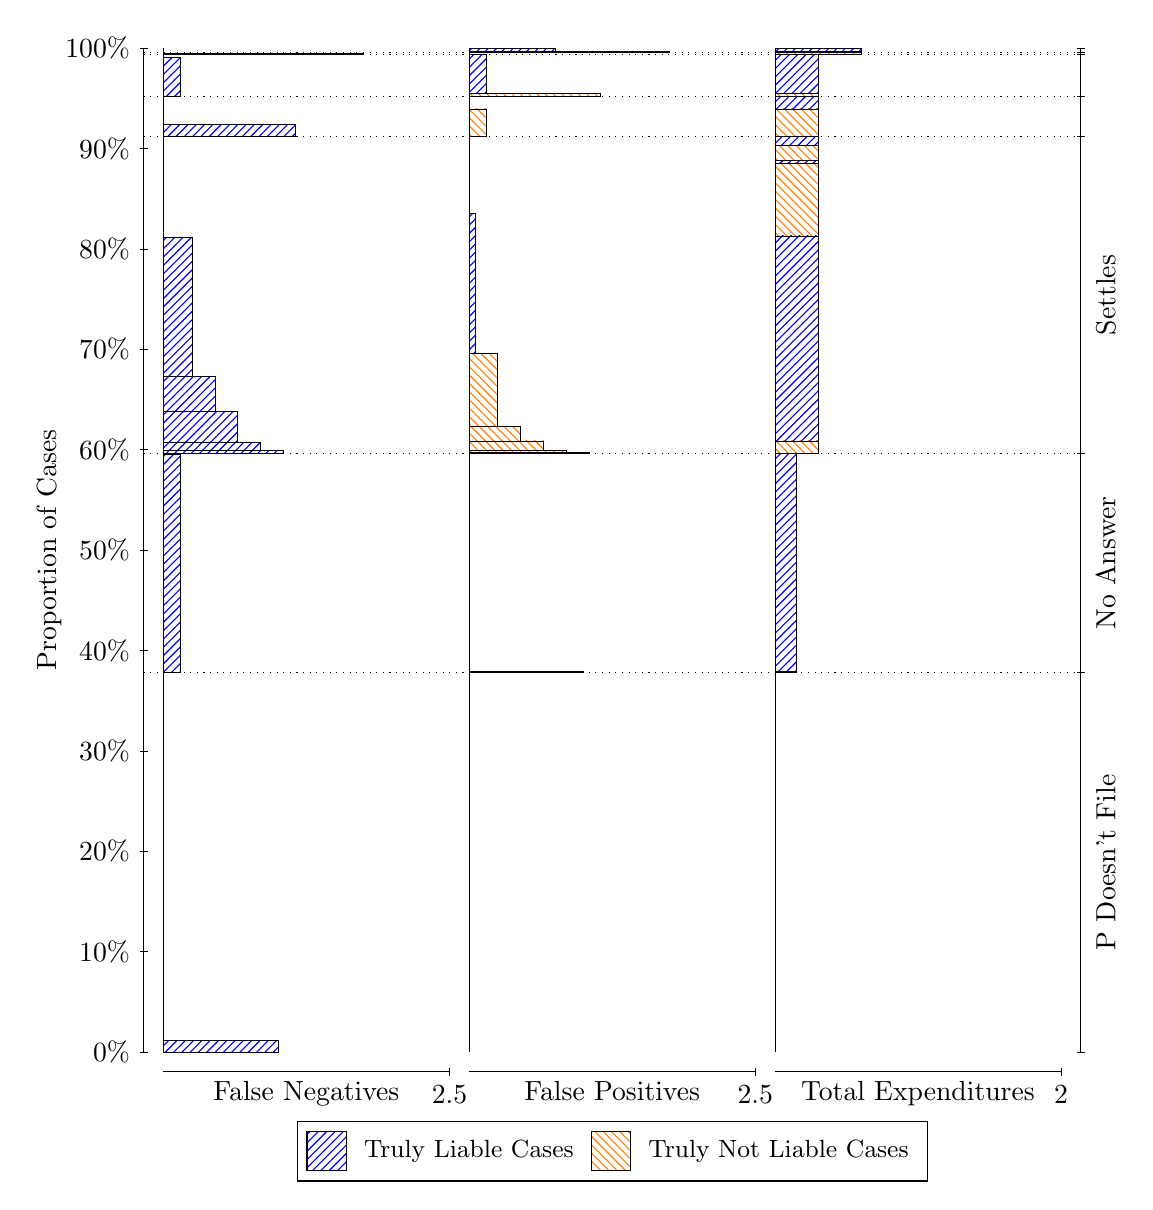
\begin{tikzpicture}
\draw[black, very thin] (1.5,1.75) -- (1.5,14.5);
\node[rotate=90, text=black, anchor=center] at (0.3, 8.125) {Proportion of Cases};
\draw[black, very thin] (1.45,1.75) -- (1.55,1.75);
\node[text=black, anchor=east] at (1.45, 1.75) {0\%};
\draw[black, very thin] (1.45,3.025) -- (1.55,3.025);
\node[text=black, anchor=east] at (1.45, 3.025) {10\%};
\draw[black, very thin] (1.45,4.3) -- (1.55,4.3);
\node[text=black, anchor=east] at (1.45, 4.3) {20\%};
\draw[black, very thin] (1.45,5.575) -- (1.55,5.575);
\node[text=black, anchor=east] at (1.45, 5.575) {30\%};
\draw[black, very thin] (1.45,6.85) -- (1.55,6.85);
\node[text=black, anchor=east] at (1.45, 6.85) {40\%};
\draw[black, very thin] (1.45,8.125) -- (1.55,8.125);
\node[text=black, anchor=east] at (1.45, 8.125) {50\%};
\draw[black, very thin] (1.45,9.4) -- (1.55,9.4);
\node[text=black, anchor=east] at (1.45, 9.4) {60\%};
\draw[black, very thin] (1.45,10.675) -- (1.55,10.675);
\node[text=black, anchor=east] at (1.45, 10.675) {70\%};
\draw[black, very thin] (1.45,11.95) -- (1.55,11.95);
\node[text=black, anchor=east] at (1.45, 11.95) {80\%};
\draw[black, very thin] (1.45,13.225) -- (1.55,13.225);
\node[text=black, anchor=east] at (1.45, 13.225) {90\%};
\draw[black, very thin] (1.45,14.5) -- (1.55,14.5);
\node[text=black, anchor=east] at (1.45, 14.5) {100\%};

\draw[black, very thin] (13.4,1.75) -- (13.4,14.5);
\draw[black, very thin] (13.35,1.75) -- (13.45,1.75);
\node[anchor=west] at (13.35, 1.75) {};
\draw[black, very thin] (13.35,6.5683) -- (13.45,6.5683);
\node[anchor=west] at (13.35, 6.5683) {};
\draw[black, very thin] (13.35,9.3524) -- (13.45,9.3524);
\node[anchor=west] at (13.35, 9.3524) {};
\draw[black, very thin] (13.35,13.374) -- (13.45,13.374);
\node[anchor=west] at (13.35, 13.374) {};
\draw[black, very thin] (13.35,13.885) -- (13.45,13.885);
\node[anchor=west] at (13.35, 13.885) {};
\draw[black, very thin] (13.35,14.421) -- (13.45,14.421);
\node[anchor=west] at (13.35, 14.421) {};
\draw[black, very thin] (13.35,14.448) -- (13.45,14.448);
\node[anchor=west] at (13.35, 14.448) {};
\draw[black, very thin] (13.35,14.5) -- (13.45,14.5);
\node[anchor=west] at (13.35, 14.5) {};

\draw[black, very thin, pattern color=blue, pattern=north east lines] (1.75,1.75) rectangle (3.2033,1.8937);
\draw[black, very thin, pattern color=orange, pattern=north west lines] (1.75,1.8937) rectangle (1.75,6.5683);
\draw[black, very thin, pattern color=blue, pattern=north east lines] (1.75,6.5683) rectangle (1.968,9.3413);
\draw[black, very thin, pattern color=orange, pattern=north west lines] (1.75,9.3413) rectangle (1.75,9.3524);
\draw[black, very thin, pattern color=blue, pattern=north east lines] (1.75,9.3524) rectangle (3.276,9.3859);
\draw[black, very thin, pattern color=blue, pattern=north east lines] (1.75,9.3859) rectangle (2.9853,9.495);
\draw[black, very thin, pattern color=blue, pattern=north east lines] (1.75,9.495) rectangle (2.6947,9.8893);
\draw[black, very thin, pattern color=blue, pattern=north east lines] (1.75,9.8893) rectangle (2.404,10.327);
\draw[black, very thin, pattern color=blue, pattern=north east lines] (1.75,10.327) rectangle (2.1133,12.1);
\draw[black, very thin, pattern color=orange, pattern=north west lines] (1.75,12.1) rectangle (1.75,13.374);
\draw[black, very thin, pattern color=blue, pattern=north east lines] (1.75,13.374) rectangle (3.4213,13.532);
\draw[black, very thin, pattern color=orange, pattern=north west lines] (1.75,13.532) rectangle (1.75,13.885);
\draw[black, very thin, pattern color=blue, pattern=north east lines] (1.75,13.885) rectangle (1.968,14.383);
\draw[black, very thin, pattern color=orange, pattern=north west lines] (1.75,14.383) rectangle (1.75,14.421);
\draw[black, very thin, pattern color=blue, pattern=north east lines] (1.75,14.421) rectangle (4.2933,14.428);
\draw[black, very thin, pattern color=orange, pattern=north west lines] (1.75,14.428) rectangle (1.75,14.448);
\draw[black, very thin, pattern color=orange, pattern=north west lines] (1.75,14.448) rectangle (1.75,14.453);
\draw[black, very thin, pattern color=blue, pattern=north east lines] (1.75,14.453) rectangle (1.75,14.5);
\draw[black, very thin, pattern color=orange, pattern=north west lines] (5.6333,1.75) rectangle (5.6333,6.4246);
\draw[black, very thin, pattern color=blue, pattern=north east lines] (5.6333,6.4246) rectangle (5.6333,6.5683);
\draw[black, very thin, pattern color=orange, pattern=north west lines] (5.6333,6.5683) rectangle (7.0867,6.5794);
\draw[black, very thin, pattern color=blue, pattern=north east lines] (5.6333,6.5794) rectangle (5.6333,9.3524);
\draw[black, very thin, pattern color=orange, pattern=north west lines] (5.6333,9.3524) rectangle (7.1593,9.3658);
\draw[black, very thin, pattern color=orange, pattern=north west lines] (5.6333,9.3658) rectangle (6.8687,9.3877);
\draw[black, very thin, pattern color=orange, pattern=north west lines] (5.6333,9.3877) rectangle (6.578,9.5097);
\draw[black, very thin, pattern color=orange, pattern=north west lines] (5.6333,9.5097) rectangle (6.2873,9.6997);
\draw[black, very thin, pattern color=orange, pattern=north west lines] (5.6333,9.6997) rectangle (5.9967,10.626);
\draw[black, very thin, pattern color=blue, pattern=north east lines] (5.6333,10.626) rectangle (5.706,12.4);
\draw[black, very thin, pattern color=blue, pattern=north east lines] (5.6333,12.4) rectangle (5.6333,13.374);
\draw[black, very thin, pattern color=orange, pattern=north west lines] (5.6333,13.374) rectangle (5.8513,13.727);
\draw[black, very thin, pattern color=blue, pattern=north east lines] (5.6333,13.727) rectangle (5.6333,13.885);
\draw[black, very thin, pattern color=orange, pattern=north west lines] (5.6333,13.885) rectangle (7.3047,13.923);
\draw[black, very thin, pattern color=blue, pattern=north east lines] (5.6333,13.923) rectangle (5.8513,14.421);
\draw[black, very thin, pattern color=orange, pattern=north west lines] (5.6333,14.421) rectangle (5.6333,14.441);
\draw[black, very thin, pattern color=blue, pattern=north east lines] (5.6333,14.441) rectangle (5.6333,14.448);
\draw[black, very thin, pattern color=orange, pattern=north west lines] (5.6333,14.448) rectangle (8.1767,14.453);
\draw[black, very thin, pattern color=blue, pattern=north east lines] (5.6333,14.453) rectangle (6.7233,14.5);
\draw[black, very thin, pattern color=orange, pattern=north west lines] (9.5167,1.75) rectangle (9.5167,6.4246);
\draw[black, very thin, pattern color=blue, pattern=north east lines] (9.5167,6.4246) rectangle (9.5167,6.5683);
\draw[black, very thin, pattern color=orange, pattern=north west lines] (9.5167,6.5683) rectangle (9.7892,6.5794);
\draw[black, very thin, pattern color=blue, pattern=north east lines] (9.5167,6.5794) rectangle (9.7892,9.3524);
\draw[black, very thin, pattern color=orange, pattern=north west lines] (9.5167,9.3524) rectangle (10.062,9.5097);
\draw[black, very thin, pattern color=blue, pattern=north east lines] (9.5167,9.5097) rectangle (10.062,12.115);
\draw[black, very thin, pattern color=orange, pattern=north west lines] (9.5167,12.115) rectangle (10.062,13.042);
\draw[black, very thin, pattern color=blue, pattern=north east lines] (9.5167,13.042) rectangle (10.062,13.075);
\draw[black, very thin, pattern color=orange, pattern=north west lines] (9.5167,13.075) rectangle (10.062,13.265);
\draw[black, very thin, pattern color=blue, pattern=north east lines] (9.5167,13.265) rectangle (10.062,13.374);
\draw[black, very thin, pattern color=orange, pattern=north west lines] (9.5167,13.374) rectangle (10.062,13.727);
\draw[black, very thin, pattern color=blue, pattern=north east lines] (9.5167,13.727) rectangle (10.062,13.885);
\draw[black, very thin, pattern color=orange, pattern=north west lines] (9.5167,13.885) rectangle (10.062,13.923);
\draw[black, very thin, pattern color=blue, pattern=north east lines] (9.5167,13.923) rectangle (10.062,14.421);
\draw[black, very thin, pattern color=orange, pattern=north west lines] (9.5167,14.421) rectangle (10.607,14.441);
\draw[black, very thin, pattern color=blue, pattern=north east lines] (9.5167,14.441) rectangle (10.607,14.448);
\draw[black, very thin, pattern color=orange, pattern=north west lines] (9.5167,14.448) rectangle (10.607,14.453);
\draw[black, very thin, pattern color=blue, pattern=north east lines] (9.5167,14.453) rectangle (10.607,14.5);
\draw[black, dotted] (1.5,6.5683) -- (13.4,6.5683);
\draw[black, dotted] (1.5,9.3524) -- (13.4,9.3524);
\draw[black, dotted] (1.5,13.374) -- (13.4,13.374);
\draw[black, dotted] (1.5,13.885) -- (13.4,13.885);
\draw[black, dotted] (1.5,14.421) -- (13.4,14.421);
\draw[black, dotted] (1.5,14.448) -- (13.4,14.448);
\draw[black, very thin] (1.75,1.5) -- (5.3833,1.5);
\node[text=black, anchor=north] at (3.5667, 1.5) {False Negatives};
\draw[black, very thin] (5.3833,1.45) -- (5.3833,1.55);
\node[text=black, anchor=north] at (5.3833, 1.45) {2.5};

\draw[black, very thin] (5.6333,1.5) -- (9.2667,1.5);
\node[text=black, anchor=north] at (7.45, 1.5) {False Positives};
\draw[black, very thin] (9.2667,1.45) -- (9.2667,1.55);
\node[text=black, anchor=north] at (9.2667, 1.45) {2.5};

\draw[black, very thin] (9.5167,1.5) -- (13.15,1.5);
\node[text=black, anchor=north] at (11.333, 1.5) {Total Expenditures};
\draw[black, very thin] (13.15,1.45) -- (13.15,1.55);
\node[text=black, anchor=north] at (13.15, 1.45) {2};

\node[text=black, centered, rotate=90] at (13.72, 4.1592) {P Doesn't File};
\node[text=black, centered, rotate=90] at (13.72, 7.9604) {No Answer};
\node[text=black, centered, rotate=90] at (13.72, 11.363) {Settles};





\draw (7.449999999999999,1.5) node[draw=none] (baseCoordinate) {};
\begin{scope}[align=center]
        \matrix[scale=0.5, draw=black, below=0.5cm of baseCoordinate, nodes={draw}, column sep=0.1cm]{
            \node[rectangle, draw, minimum width=0.5cm, minimum height=0.5cm, pattern color=blue, pattern=north east lines] {}; &
            \node[draw=none, font=\small, text=black] (B) {Truly Liable Cases}; &
            \node[rectangle, draw, minimum width=0.5cm, minimum height=0.5cm, pattern color=orange, pattern=north west lines] {}; &
            \node[draw=none, font=\small, text=black] (B) {Truly Not Liable Cases}; \\
            };
\end{scope}

\end{tikzpicture}
\end{document}